%% LyX 2.0.5.1 created this file.  For more info, see http://www.lyx.org/.
%% Do not edit unless you really know what you are doing.
\documentclass[11pt,dutch]{article}
\usepackage[T1]{fontenc}
\usepackage[a4paper]{geometry}
\geometry{verbose,tmargin=3cm,bmargin=3cm,lmargin=2cm,rmargin=2cm}
\usepackage{fancyhdr}
\pagestyle{fancy}
\setlength{\parskip}{\smallskipamount}
\setlength{\parindent}{0pt}
\usepackage{array}
\usepackage{amsmath}
\usepackage{amssymb}
\usepackage{graphicx}
\usepackage{setspace}
\setstretch{1.2}

\makeatletter

%%%%%%%%%%%%%%%%%%%%%%%%%%%%%% LyX specific LaTeX commands.
%% Because html converters don't know tabularnewline
\providecommand{\tabularnewline}{\\}

\@ifundefined{date}{}{\date{}}
%%%%%%%%%%%%%%%%%%%%%%%%%%%%%% User specified LaTeX commands.


\usepackage[dutch]{babel}


\usepackage{fouriernc}\usepackage[detect-all,load-configurations=binary,separate-uncertainty=true,per-mode=symbol]{siunitx}










\numberwithin{equation}{section}
\numberwithin{figure}{section}

\graphicspath{{Figures/}}

\usepackage{fancyhdr}
\fancyhf{}
\rhead{\thepage}
\renewcommand{\footrulewidth}{0pt}
\renewcommand{\headrulewidth}{0pt}

\newcommand{\hisparc}{\textsmaller{HiSPARC}\xspace}
\newcommand{\kascade}{\textsmaller{KASCADE}\xspace}
\newcommand{\sapphire}{\textsmaller{SAPPHiRE}\xspace}
\newcommand{\jsparc}{\textsmaller{jSparc}\xspace}
\newcommand{\hdf}{\textsmaller{HDF5}\xspace}
\newcommand{\aires}{\textsmaller{AIRES}\xspace}
\newcommand{\csv}{\textsmaller{CSV}\xspace}
\newcommand{\python}{\textsmaller{PYTHON}\xspace}
\newcommand{\corsika}{\textsmaller{CORSIKA}\xspace}
\newcommand{\labview}{\textsmaller{LabVIEW}\xspace}
\newcommand{\daq}{\textsmaller{DAQ}\xspace}
\newcommand{\adc}{\textsmaller{ADC}\xspace}
\newcommand{\hi}{\textsc{h i}\xspace}
\newcommand{\hii}{\textsc{h ii}\xspace}
\newcommand{\mip}{\textsmaller{MIP}\xspace}
\newcommand{\hisparcii}{\textsmaller{HiSPARC II}\xspace}
\newcommand{\hisparciii}{\textsmaller{HiSPARC III}\xspace}

\DeclareSIUnit{\electronvolt}{\ensuremath{\mathrm{e\!\!\:V}}}

\DeclareSIUnit{\unitsigma}{\ensuremath{\sigma}}
\DeclareSIUnit{\mip}{\textsmaller{MIP}}
\DeclareSIUnit{\adc}{\textsmaller{ADC}}

\DeclareSIUnit{\gauss}{G}
\DeclareSIUnit{\parsec}{pc}
\DeclareSIUnit{\year}{yr}

\makeatother

\usepackage{babel}
\usepackage{xunicode}
\begin{document}

\title{Pulshoogte en pulsintegraal}


\author{A. de Laat, N.G. Schultheiss}

\maketitle

\section{Inleiding}

De detectoren van een HiSPARC-station zijn uitgerust met PhotoMultiPlier
(PMT) buizen. Als er geen deeltjes door de detector schiten, treedt
er geen fluoriscentie op en is er geen licht. Bijgevolg geeft de PMT-buis
een electrisch signaal van 0mv aan de HiSPARC II of HiSPARC III box.
In de box wordt het analoge signaal door middel van een Analoog Digitaal
Converter (ADC) omgezet in een digitaal signaal. De grootte van dit
signaal wordt uitgedrukt in ADCs, in dit geval gaat het om een getal
zonder eenheid, de Analog Digital Count.

Als er een signaal gemeten wordt, wordt en reeks van deze ADCs in
de HiSPARC box opgeslagen. Als er tegelijkertijd een tweede reeks
wordt opgeslagen worden deze reeksen ADCs naar de HiSPARC server gezonden.
Een dergelijke reeks ADCs vormt een puls. Deze pulsen worden ingedeeld
naar de pulshoogte en de pulsintegraal (het pulsoppervlak).


\section{De pulsvorm}


\subsection{Pulsen ophalen uit de HiSPARC data opslag}

In de praktijk kunnen we een set pulsen voor een willekeurige gebeurtenis
ophalen met jSparc%
\footnote{Het interactieve practicum jSparc kan in de les worden via de aanvraag
van een sessie worden gebruikt, het is ook mogelijk om een willekeurige
set pulsen op te halen op: \texttt{http://data.hisparc.nl/media/jsparc/jsparc.html}.%
}. In deze module gaan we uit van de set pulsen die met de stations
uit figuur \ref{fig:coincidence} zijn gemeten.

\begin{figure}[h]
\noindent \begin{centering}
\begin{tabular}{cc}
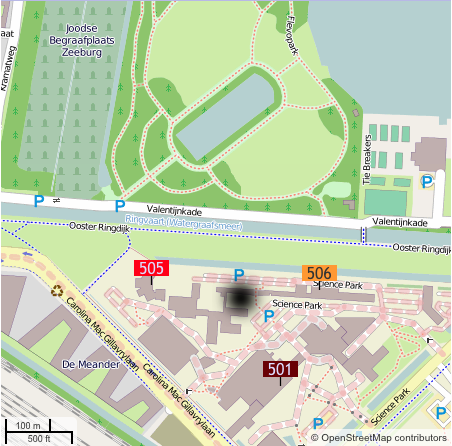
\includegraphics[scale=0.33]{Figures/kaart} & 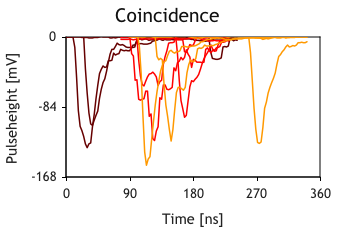
\includegraphics[scale=0.65]{Figures/Coincidence}\tabularnewline
\end{tabular}
\par\end{centering}

\caption{\label{fig:coincidence}De plattegrond met de locaties van de meetstations
en de gemeten pulsen per station.}
\end{figure}


Op de kaart zijn drie meetstations te zien, een rood, een bruin, een
rood en een oranje station%
\footnote{De kleuren van de stations volgen de definitie van de kleurcode van
weerstandjes: bruin: 1, rood: 2, oranje: 3, geel: 4, groen: 5, blauw:
6, violet: 7, etc. %
}. We zien dat alle stations een aantal pulsen hebben gegeven. Dit
komt omdat een station uit meerdere detectoren bestaat.


\subsection{Eenvoudige pulsvormen}

\begin{figure}[h]
\noindent \begin{centering}
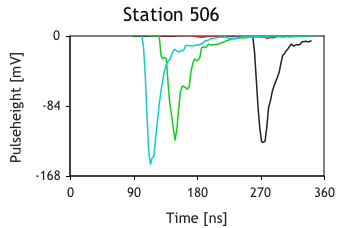
\includegraphics[scale=0.65]{Figures/Traces506}
\par\end{centering}

\caption{\label{fig:Eenvoudige-pulsen}Eenvoudige pulsen}
\end{figure}


In figuur \ref{fig:Eenvoudige-pulsen} zijn de sigalen van vier detectoren
te zien. De zwarte puls van detector 1 heeft een vrij snelle voorflank.
Het verloop van de achterflank lijkt een halfwaardetijd te hebben
(deze loopt exponentieël op). Bij de blauwe grafiek van detector 4
is iets soortgelijks aan de hand. 


\paragraph{Opdracht 1:}

\textit{Leg uit wat je kunt zeggen over de groene grafiek van detector
3. }

\begin{tabular}{>{\centering}p{17cm}}
\tabularnewline
\hline 
\tabularnewline
\hline 
\tabularnewline
\hline 
\tabularnewline
\hline 
\end{tabular}

\smallskip{}


Meestal zien de grafieken er niet zo mooi uit als in figuur \ref{fig:Eenvoudige-pulsen}.
In figuur \ref{fig:Iets-complexere-pulsen} zijn de pulsen van detector
1 en 4 goed te zien (respectievelijk zwart en blauw).

\begin{figure}[h]
\noindent \begin{centering}
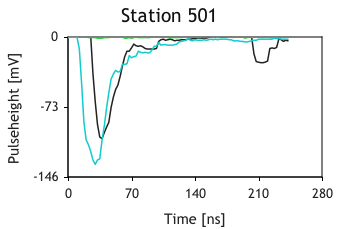
\includegraphics[scale=0.65]{Figures/Traces501}
\par\end{centering}

\caption{\label{fig:Iets-complexere-pulsen}Iets complexere pulsen}
\end{figure}



\paragraph{Opdracht 2:}

\textit{Leg uit hoe de grafiek van detector 1 in figuur \ref{fig:Iets-complexere-pulsen}
te verklaren is.}

\begin{tabular}{>{\centering}p{17cm}}
\tabularnewline
\hline 
\tabularnewline
\hline 
\tabularnewline
\hline 
\tabularnewline
\hline 
\end{tabular}


\paragraph{Opdracht 3:}

\textit{Bereken de afstand tussen de waargenomen deeltjes in de grafiek
van detector 1 in figuur \ref{fig:Iets-complexere-pulsen}.}

\begin{tabular}{>{\centering}p{17cm}}
\tabularnewline
\hline 
\tabularnewline
\hline 
\tabularnewline
\hline 
\tabularnewline
\hline 
\end{tabular}


\subsection{Ingewikkelde pulsvormen}

\begin{figure}[h]
\noindent \begin{centering}
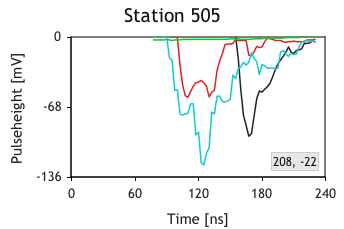
\includegraphics[scale=0.65]{Figures/Traces505}
\par\end{centering}

\caption{\label{fig:Ingewikkelde-pulsvormen}Ingewikkelde pulsvormen}
\end{figure}


Dichtbij de zwarte vlek in het kaartje van figuur \ref{fig:coincidence}
treffen we meer deeltjes aan, hoe verder je van de zwarte vlek afkomt
hoe minder deeltjes er zijn. Het aantal deeltjes per vierkante meter
kan met de NKG-functie (van Nishimura, Kamata en Greisen) worden beschreven.


\paragraph{Opdracht 4:}

\textit{Leg uit met verloop van de pulsen uit dat het midden van de
air-shower in de buurt van station 505 is.}

\begin{tabular}{>{\centering}p{17cm}}
\tabularnewline
\hline 
\tabularnewline
\hline 
\tabularnewline
\hline 
\tabularnewline
\hline 
\end{tabular}

Het valt op dat detector 3 (groen) bijna geen puls geeft.


\paragraph{Opdracht 5:}

\textit{Verklaar waarom er binnen een station soms detectoren zijn
die veel meten terwijl ander detectoren (bijna) niets meten.}

\begin{tabular}{>{\centering}p{17cm}}
\tabularnewline
\hline 
\tabularnewline
\hline 
\tabularnewline
\hline 
\tabularnewline
\hline 
\end{tabular}
\end{document}
